\chapter*{Appendix}
% The asterisk prevents this file from being labelled
% as a 'chapter.'
\section*{A.1 Bose-Einstein Distribution Derivation}
Starting with Equations 1.4 and 1.5, the average number of bosons occupying an energy state $s$ can be derived. 
\beq
P_s(n) = \frac{1}{\mathrm{Z}} e^{-n(\epsilon_s-\mu) /kT}\tag{1.4}
\eeq
\beq
\mathrm{Z}= \frac{1}{1- e^{-(\epsilon_s-\mu) /kT}}\tag{1.5}
\eeq
\begin{align*}
    \bar{n}_s = \sum_n{nP_s(n)} 
\end{align*}
For ease in notation, let's define a variable $x$, $x = \frac{(\epsilon_s-\mu) }{kT}$.
\begin{align*}
P_s(n) = \frac{1}{\mathrm{Z}} e^{-nx} 
\end{align*}
\begin{align*}
\bar{n}_s &= \sum_n{n\frac{1}{\mathrm{Z}} e^{-nx}}  \\
&= \frac{1}{\mathrm{Z}} \sum_n{ne^{-nx}} \\
&= -\frac{1}{\mathrm{Z}} \sum_n{\frac{\partial}{\partial x}e^{-nx}}
\end{align*}
As $\sum_n{}$ and $\frac{\partial}{\partial x}$ are both linear operators, they commute.
\begin{align*}
\bar{n}_s &=-\frac{1}{\mathrm{Z}} \frac{\partial}{\partial x}\sum_n{e^{-nx}} \\
\end{align*}
Under our new definition for $P_s(n)$, using $x= \frac{(\epsilon_s-\mu) }{kT}$, we find that 
\begin{align*}
    \Zeta &= \sum_n{e^{-nx}}
\end{align*}
Substituting this partition function into our equation for the average number of bosons in state $s$, we have created an expression for $\bar{n}_s$ that no longer contains an infinite sum. 
\begin{align*}
    \bar{n}_s &=-\frac{1}{\mathrm{Z}} \frac{\partial \Zeta}{\partial x}
\end{align*}
We can continue to solve using our previous definition for the partition function, substituting in $x = \frac{(\epsilon_s-\mu) }{kT}$
\beq
\mathrm{Z}= \frac{1}{1- e^{-(\epsilon_s-\mu) /kT}}\tag{1.5}
\eeq
\begin{align*}
    \mathrm{Z}&= \frac{1}{1- e^{-x}}\\
    \bar{n}_s &=-(1- e^{-x}) \frac{\partial }{\partial x}\left( \frac{1}{1- e^{-x}}\right) \\
    &= -(1- e^{-x}) (1- e^{-x})^{-2}(e^{-x})\\
    &= \frac{e^{-x}}{1-e^{-x}} \\
    &= \frac{1}{\frac{1}{e^{-x}}-1} \\
    \bar{n}_s  &= \frac{1}{e^x-1}\tag{1.6}
\end{align*}
The equation above is \textbf{Equation 1.6}, substituting in $x$. This equation is known as the Bose-Einstein distribution. 
\newpage

\section*{A.2 Rubidium-87 Energy Levels}

\begin{figure}[t]
\begin{center}
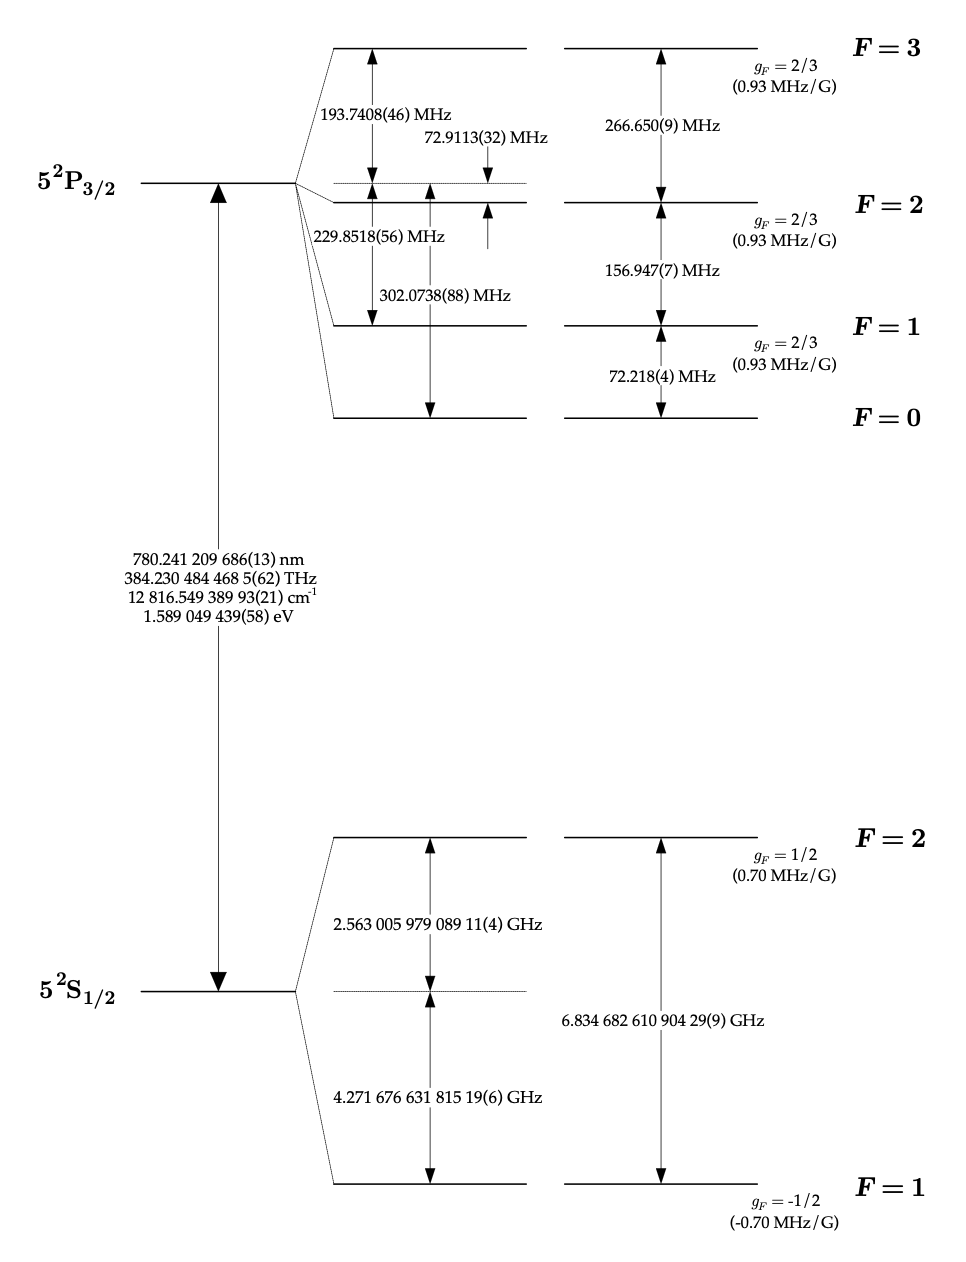
\epsfig{file=fig_rb_energy.png, scale = .9}
\end{center}
\end{figure}
\textbf{Figure A.1} The energy levels of Rubidium-87 and Land\'e factors. \cite{steck} 

\section*{A.3 Optical Pumping Simulation Code}
This code is written in python. 
\newline
\inputminted[fontsize=\footnotesize, frame=leftline, linenos]{python}{optical_pumping.py}

\endinput

